\documentclass{article}
\usepackage{graphicx}
\usepackage{amsmath}
\usepackage[T2A]{fontenc}  % For Cyrillic fonts
\usepackage[utf8]{inputenc}  % For UTF-8 encoding
\usepackage[russian,english]{babel}  % For Russian language support
\usepackage{amssymb}
\usepackage[margin=2cm]{geometry}
\usepackage{listings}
\usepackage{xcolor}
\usepackage{float}
\usepackage{hyperref}

\lstset{
    language=Python,
    basicstyle=\ttfamily\small,
    keywordstyle=\color{blue},
    stringstyle=\color{red},
    commentstyle=\color{gray},
    backgroundcolor=\color{lightgray!20},
    frame=single,
    rulecolor=\color{black},
    numbers=left,
    numberstyle=\tiny\color{gray},
    stepnumber=1,
    numbersep=10pt,
    showspaces=false,
    showstringspaces=false,
    breaklines=true,
    breakatwhitespace=true,
    tabsize=4,
    captionpos=b
}

\title{Математическая статистика \\ Домашнее задание 1}
\author{Никита Загайнов}

\date{\today}

\begin{document}

\maketitle

\begin{enumerate}
	\item
	      Эффективная оценка - это оценка, дисперсия которой
	      достигает границы Крамера-Рао:
	      \[
		      \Variance(\widehat{\theta}) = \frac{1}{ni(\theta)}
	      \]
	      Она достигается в случае, если оценка является несмещённой,
	      её функция плотности дифференцируема по оцениваемому параметру,
	      её область определения не зависит от оцениваемого параметра,
	      для любого $\theta$ существует информация Фишера, и распредение
	      принадлежит экспоненциальному семейству.
	      Функцию плотности из экспоненциального семейства можно записать
	      следующим образом:
	      \[
		      f(x, \theta) = h(x) \exp\left(
		      \sum_{i=1}^k a_i(\theta) f_i(x) + b_i(\theta) \right)
	      \]
	      Докажем, что нормальное распределение принадлежит экспоненциальному
	      семейству.
	      Функция плотности нормального распределения:
	      \begin{equation*}
		      \begin{aligned}
			      f(x, \alpha, \sigma^2) & = \frac{1}{\sqrt{2\pi\sigma^2}}
			      \exp\left(-\frac{(x - \alpha)^2}{2\sigma^2}\right)                                               \\
			                             & = \frac{\exp \left( -\frac{1}{2\sigma^2} \right) }{\sqrt{2\pi\sigma^2}}
			      \exp\left( x^2 + 2\alpha x + \alpha^2 \right)                                                    \\
		      \end{aligned}
	      \end{equation*}
	      Подставив
	      \begin{equation*}
		      \begin{aligned}
			      h(x)        & = \frac{\exp \left( -\frac{1}{2\sigma^2} \right) }{\sqrt{2\pi\sigma^2}} &             &           \\
			      f_1(x)      & = x^2                                                                   & a_1(\alpha) & = 1       \\
			      f_2(x)      & = x                                                                     & a_2(\alpha) & = 2\alpha \\
			      b_1(\alpha) & = \alpha^2                                                              & b_2(\alpha) & = 0       \\
		      \end{aligned}
	      \end{equation*}

	      Получим, что нормальное распределение
	      принадлежит экспоненциальному семейству.

	      Проверим выполнение условий регулярности:
	      \begin{enumerate}
		      \item Среднее по выборке - несмещённая оценка для $\alpha$
		      \item Функция плотности дифференцируема по $\alpha$:
		            \[
			            \frac{\partial}{\partial \alpha} 
                        f(x, \alpha, \sigma^2) = 
                        \frac{1}{\sqrt{2\pi\sigma^2}} 
                        \frac{x - \alpha}{\sigma^2} 
                        \exp\left(-\frac{(x - \alpha)^2}{2\sigma^2}\right)
		            \]
		      \item Область определения: $x \in (-\infty, \infty)$
		      \item Информация Фишера существует:
		            \[
			            i(\alpha) = 
                        -\mathbb{E}\left(\frac{\partial^2}
                        {\partial \alpha^2} \ln 
                        f(x, \alpha, \sigma^2)\right) = 
                        \frac{1}{\sigma^2}
		            \]
	      \end{enumerate}

	      Тогда среднее по выборке является эффективной оценкой
	      для $\alpha$.

	\item Оценка
	      \[
		      \widehat{\sigma}^2 = \frac{1}{n} \sum_{i}^{n}
	      \]
	      является несмещённой оценкой для $\sigma^2$:
	      \begin{equation*}
		      \begin{aligned}
			      \mathbb{E}( \widehat{\sigma}^2 )
			       & = \mathbb{E}\left( \frac{1}{n} \sum_{i}^{n} X_i^2 \right)  = \frac{1}{n} \sum_{i}^{n} \mathbb{E}(X_i^2) = \frac{1}{n} \sum_{i}^{n} \sigma^2 = \sigma^2
		      \end{aligned}
	      \end{equation*}

	      Подставив в функцию плотности нормального распределения
	      \begin{equation*}
		      \begin{aligned}
			      h(x)   & = \frac{\exp \left( -\frac{x^2}{2} \right) }{\sqrt{2\pi}} &               &                      &               &                         \\
			      f_1(x) & = 1                                                       & a_1(\sigma^2) & = \frac{1}{\sigma^2} & b_1(\sigma^2) & = \ln{\frac{1}{\sigma}} \\
		      \end{aligned}
	      \end{equation*}
	      Получим, что это распределение принадлежит экспоненциальному семейству.
	      Проверим условия регулярности:
	      \begin{enumerate}
		      \item Оценка несмещённая
		      \item Функция плотности дифференцируема по $\sigma^2$:
                    \[
                        \frac{\partial}{\partial (\sigma^2)} f(x, \sigma^2) =
                        -\frac{1}{2\sqrt{2 \pi} \sigma^3} \exp\left(-\frac{x^2}{2\sigma^2}\right) +
                        \frac{x^2}{2\sqrt{2 \pi} \sigma^5} \exp\left(-\frac{x^2}{2\sigma^2}\right)
                    \]
		      \item Область определения: $x \in (-\infty, \infty)$
		      \item Информация Фишера существует:
		            \[
			            i(\sigma^2) =
			            -\mathbb{E}\left(\frac{\partial^2}{\partial
				            (\sigma^2)^2} \ln f(x, \sigma^2)\right) =
			            \frac{1}{2\sigma^4}
		            \]
	      \end{enumerate}

	      Тогда оценка является эффективной.


	\item Применим теорему Леманна-Шеффе. Функция плотности для
	      выборки:
	      \[
		      p(X, 0, \theta) =
		      \prod_{i=1}^n \frac{1}{\theta} I(X_i \in [0, \theta]) =
		      \frac{1}{\theta^n} I(X_{(n)} \leq \theta)
	      \]
	      Где $X_{(n)} = \max(X)$.
	      Выберем статистику $T(X) = X_{(n)}$, тогда плотность принимает
	      вид $p(X, \theta) = \frac{1}{\theta^n} I(T(X) \leq \theta)$,
	      что значит, что $T(X)$ является достаточной статистикой.
	      Эта статистика также является полной. Для доказательства
	      найдём функцию плотности для $T(X)$:
	      \begin{equation*}
		      \begin{aligned}
			      P(T \leq x)     & = P(X_{(n)} \leq x) = P(\max(X) \leq x) =                                  \\
			                      & = \prod_{i=1}^n P(X_i \leq x) = F(x)^n = \left( \frac{x}{\theta} \right)^n \\
			      p(x, n, \theta) & = \frac{d}{dx} P(T \leq x) = \frac{n}{\theta^n} x^{n-1}
		      \end{aligned}
	      \end{equation*}
	      Проверим, что статистика $T(X)$ является полной:
	      \begin{equation*}
		      \begin{aligned}
			      \mathbb{E}g(T)      & = \int_0^\theta g(x) \frac{n}{\theta^n} x^{n-1} dx                                     \\
			                          & = \frac{n}{\theta^n} \int_0^\theta g(x) x^{n-1} dx = 0, \forall \theta \Longrightarrow \\
			      G                   & = \int_0^\theta g(x) x^{n-1} dx = 0, \forall \theta \iff                               \\
			      \frac{d}{d\theta} G & = g(x) x^{n-1} = 0, \forall \theta \iff                                                \\
			      g(T)                & = 0, \forall \theta
		      \end{aligned}
	      \end{equation*}

	      Тогда мы можем применить теорему Леманна-Шеффе,
	      чтобы получить оптимальную оценку. Для этого приравняем
	      математическое ожидание функции от статистики к $\theta$:

	      \begin{equation*}
		      \begin{aligned}
			       & \mathbb{E}g(T) = \theta \iff                                   \\
			       & \int_0^\theta g(x) \frac{n}{\theta^n} x^{n-1} dx = \theta \iff \\
			       & \int_0^\theta g(x) x^{n-1} dx = \frac{\theta^{n+1}}{n} \iff    \\
			       & g(x) = \frac{n+1}{n} x
		      \end{aligned}
	      \end{equation*}

	      Тогда оптимальной оценкой для $\theta$ является
	      \[
		      \widehat{\theta} = \frac{n+1}{n} X_{(n)}
	      \]

	\item
	      \begin{enumerate}
		      \item[(a)] Метод моментов для распределения $U(a, b)$:
			      \begin{align*}
				       & f_1(a, b) = \frac{1}{n} \sum_{i=1}^n X_i   \\
				       & f_2(a, b) = \frac{1}{n} \sum_{i=1}^n X_i^2 \\
			      \end{align*}
			      Для равномерного распределения известны среднее и дисперсия:
			      \[
				      E(X) = \frac{a + b}{2}, \quad \Variance(X) = \frac{(b - a)^2}{12}
			      \]
			      Подставим их в метод:

			      \begin{align*}
				       & \frac{a + b}{2} = \frac{1}{n} \sum_{i=1}^n X_i                              \\
				       & \frac{(b - a)^2}{12} = \frac{1}{n} \sum_{i=1}^n X_i^2 - \frac{(a + b)^2}{4}
			      \end{align*}

			      Откуда выражаем:
			      \begin{align*}
				       & a = \frac{1}{n} \sum_{i=1}^n X_i - \sqrt{3} \sqrt{\frac{1}{n} \sum_{i=1}^n X_i^2 - \left(\frac{1}{n} \sum_{i=1}^n X_i\right)^2} \\
				       & b = \frac{1}{n} \sum_{i=1}^n X_i + \sqrt{3} \sqrt{\frac{1}{n} \sum_{i=1}^n X_i^2 - \left(\frac{1}{n} \sum_{i=1}^n X_i\right)^2}
			      \end{align*}

		      \item[(b)]
			      Следующий код был использован для тестирования метода:
			      \begin{lstlisting}
from typing import Tuple
import numpy as np
from matplotlib import pyplot as plt


def get_estimates(data: np.ndarray) -> Tuple[np.ndarray, np.ndarray]:
    first_moment = np.mean(data, axis=1)
    second_moment = np.mean(data * data, axis=1)

    subtrahend = np.sqrt(3) * np.sqrt(second_moment - first_moment * first_moment)
    a = first_moment - subtrahend
    b = first_moment + subtrahend
    return a, b


def main():
    ns = np.logspace(1, 5, 10, dtype=int)
    trials = 1000

    a_true = -np.exp(2)
    b_true = np.pi * 2.5

    plt.figure(figsize=(10, 6))

    errors_a = []
    errors_b = []
    for n in ns:
        samples = np.random.uniform(a_true, b_true, (trials, n))
        a_est, b_est = get_estimates(samples)
        errors_a.append(np.mean((a_est - a_true) ** 2))
        errors_b.append(np.mean((b_est - b_true) ** 2))

    plt.plot(ns, errors_a, "o-", label="Error of a")
    plt.plot(ns, errors_b, "o-", label="Error of b")
    plt.xlabel("n")
    plt.ylabel("MSE")
    plt.legend()
    plt.grid()
    plt.yscale("log")
    plt.xscale("log")

    plt.savefig("task4.png")


if __name__ == "__main__":
    main()

                \end{lstlisting}

			      На выходе получен график \ref{fig:task4}.
			      \begin{figure}[H]
				      \centering
				      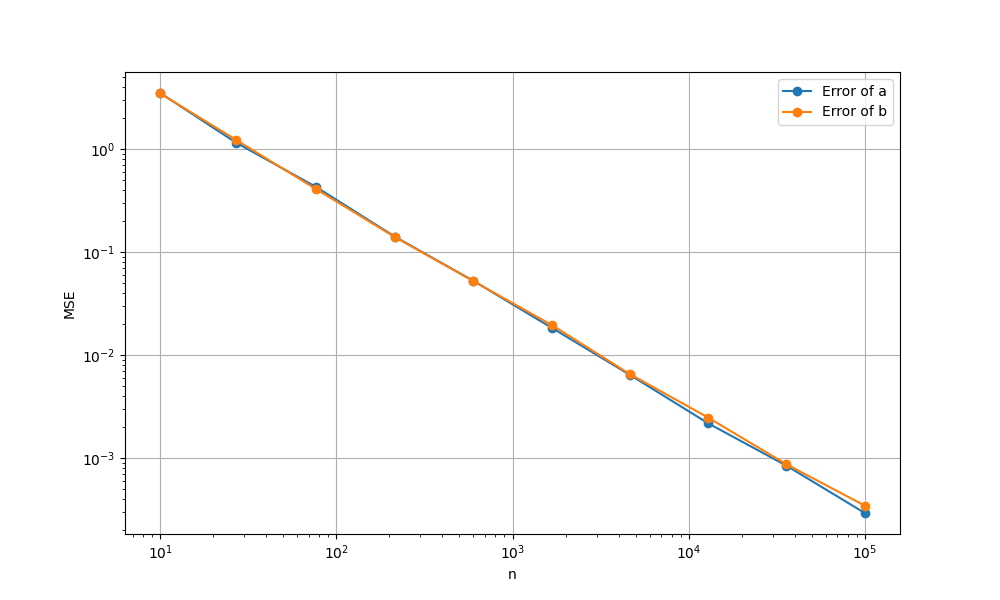
\includegraphics[width=0.8\textwidth]{task4.png}
				      \caption{Зависимость среднеквадратичной ошибки от размера выборки}
				      \label{fig:task4}
			      \end{figure}

	      \end{enumerate}

	\item Запишем функцию правдоподобия для
	      данного распределения на выборке $X_1, \ldots, X_n$:
	      \[
		      p(X, \alpha) = \prod_{i=1}^n \alpha
		      \exp(\alpha (X_i - \beta))
	      \]
	      Прологарифмируем её:

	      \[
		      \ln p(X, \alpha) = n \ln \alpha - n \beta + \alpha \sum_{i=1}^n (X_i)
	      \]

	      Приравняем градиент к нулю:
	      \begin{align*}
		       & \frac{\partial}{\partial \alpha} \ln p(X, \alpha) = 0 \\
		       & \frac{n}{\alpha} - n \beta + \sum_{i=1}^n X_i = 0     \\
		       & \alpha = \frac{n}{n \beta + \sum_{i=1}^n X_i}
	      \end{align*}

	      Тогда состоятельной оценкой для $\alpha$ является
	      \[
		      \widehat{\alpha} = \frac{n}{n \beta + \sum_{i=1}^n X_i}
	      \]

	\item Запишем функцию правдоподобия:
	      \[
		      p(X, \theta) = \prod_{i=1}^n \frac{1}{5} I(X_i \in [\theta, \theta + 5])
	      \]
	      Прологарифмируем её:
	      \[
		      \ln p(X, \theta) = n \ln \frac{1}{5} + \sum_{i=1}^n I(X_i \in [\theta, \theta + 5])
	      \]
	      Получившаяся функция недиффиренцируема,
	      так что метод неприменим сам по себе. Но эту функцию
	      можно максимизировать неградиентным методом: Возьмём
	      $\theta = X_{(1)}$, тогда каждый элемент суммы будет
	      равен $1$, так как такая оценка гарантированно даст,
	      что все элементы входят в интервал $[\theta, \theta + 5]$

	      Тогда состоятельной оценкой для $\theta$ является
	      \[
		      \widehat{\theta} = X_{(1)}
	      \]

\end{enumerate}


\end{document}
